\section{MDL Beyond a Single Shard is Hard}
\label{sec:mdl:zookeeper}

\todo{\mdl{} isn't local is part of the explanation of why there are no cross-shard implementation.}

\todo{Change to 'do existing systems provide \mdl{}. Say we have a new consistency model. Do existing provide it? Surprisingly it appears single-shard implementations do not, though there is a design for it on a single shard. Then structure single-shard \mdl{} and multi-shard \mdl{}.}

There are several existing systems that could be used to implement
\multidispatch{} linearizability on a single shard. In this section,
we briefly describe them and then show how they fail to extend to
multiple shards.

\begin{figure}[!tb]
    \centering
    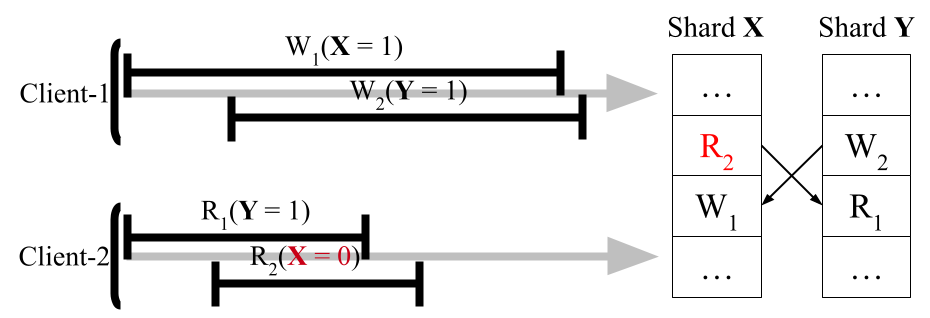
\includegraphics[width=\linewidth]{figs/somet.png}
    \caption{Example where two concurrent client processes each submit two concurrent operations. Keys \textbf{X} and \textbf{Y} are at different shards. It is possible that $R_2$ arrives before $W_1$ at shard \textbf{X}, and $W_2$ arrives before $R_1$ at shard \textbf{Y}. Since \MDL{} requires operations to take effect in invocation order, if $R_1$ returns 1, then $W_1$ must take effect before $R_1$, so $R_2$ must also return 1.}
    \label{fig:concurrentbatches}
\end{figure}

To the best of our knowledge, Zookeeper~\cite{hunt2010zookeeper} is the
only existing work to account for (in its consistency model) an 
application process potentially issuing multiple operations concurrently. The authors denote it Asynchronous Linearizability
(or A-Linearizability)~\cite{hunt2010zookeeper}. But despite its name,
it differs from \MDL{} because Zookeeper allows
reads to return stale (i.e., non-linearizable) values.

\wl{This needs to be updated to mention Diego Ongaro's dissertation as well.}

\true{To handle concurrent operations from the same process, Zookeeper uses
per-process sequence numbers.} Sequence numbers are assigned in the client 
library and increase monotonically. This provides sufficient information for
the leader to ensure each process's operations enter the log in an
order consistent with its issue order
(e.g., by queuing operations in sequence-number order).
This technique could be used with existing leader-based replicated-state-machine
protocols~\cite{ongaro2014raft,lamport1998paxos,oki1988vr} to guarantee
MDL on one shard.\footnote{Zookeeper can be forced to
guarantee \MDL{} by issuing a \texttt{sync} operation before each read to prevent it from returning a stale value.}

%\subsection{Why is this hard?}
But these protocols fail to 
guarantee \MDL{} across multiple shards for two reasons: First,
As mentioned, multiple shards
introduces the possibility for independent failures of operations. A first
operation at one shard may fail and need to be retried (e.g., due to
leader failure) while a second operation at another shard succeeds, and
its effects become visible to other processes. If both of these
operations were issued concurrently from the same process, 
this would violate \MDL{}'s suffix-closed failure semantics.

Second, allowing shards to order operations independently can lead to
violations of \MDL{}'s total order guarantee. For example, consider the
case shown in Figure~\ref{fig:concurrentbatches}. Two processes each issue two
operations, one to key $X$ and the other to key $Y$, which reside on different
shards. Process 1 writes $X$ then $Y$, and process 2 reads $Y$ then $X$. Suppose $W_2$ precedes $R_1$ at shard $Y$, causing it to return $Y=1$. Combined with
process 2's issue-order, this implies $R_2$ must be serialized after $W_1$.
But since operations can arrive at the shards in an arbitrary order, $R_2$ may
precede $W_1$ and return $X=0$, violating \MDL{}.
\wl{The numbering, capitalization, etc should be unified between this example and the examples in Section 2. Maybe }

%In the next section, we describe our new protocol, \sys{}, that tackles these
%challenges and guarantees \multidispatch{} linearizability for a multi-shard
%system.
%